\documentclass[10pt]{article}
\usepackage[a4paper,margin=1in]{geometry}
\usepackage{array}
\usepackage{graphicx}
\usepackage{xcolor}
\usepackage{longtable}
\usepackage{float}

\begin{document}

\begin{center}
  \Large \textbf{Methods of Computer Science Education: Design} \\
  \normalsize Wintersemester 2024/25 \\
  \normalsize Fabian Stiewe
\end{center}

\begin{figure}[h]
  \begin{center}
    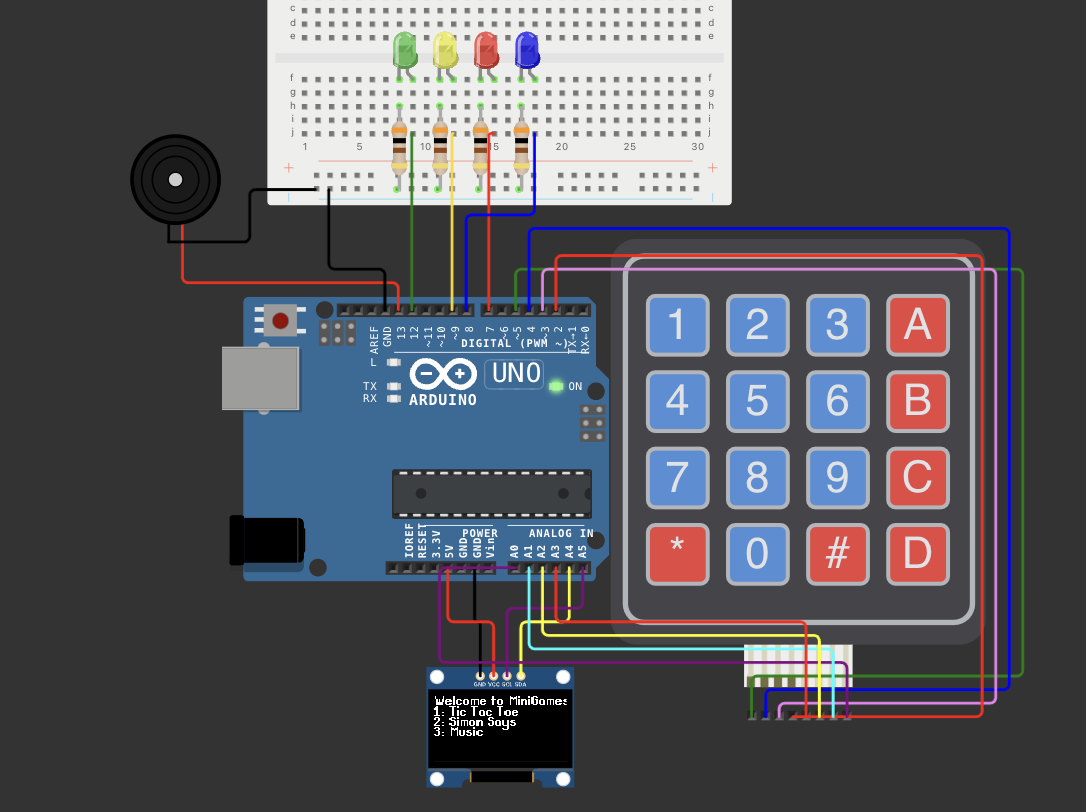
\includegraphics[width=0.6\textwidth]{diagram.png}
  \end{center}
\end{figure}

\begin{longtable}{|p{3.5cm}|p{11cm}|}
  \hline
  \textbf{Project name} & \textbf{Mini Games} using Arduino  \\ \hline
  
  \textbf{Coding files / How to use} & All necessary files for uploading the current game should be located inside the \texttt{src} or \texttt{sketch} folder. All other games, which are programmed, but currently unused can be placed inside the \texttt{otherGameList} folder. \textcolor{red}{Don't worry about errors there, it only works inside the \textbf{sketch} folder.} If you want to play a specific game, copy all necessary files into the \texttt{sketch} folder and paste the source code into the \textbf{sketch.ino} file. Only include the file, \textbf{mandatory} files for this specific game. \\ \hline
  
  \textbf{Storyline} & It is simple and quick to develop diverse games for the Arduino. This project includes the classic TicTacToe game, the known SimonSaysGame and a music player. 
  \begin{itemize}
    \item TicTacToe a simple two-player game where players take turns marking a 3x3 grid with their respective symbols (usually X and O). The objective is to be the first to get three of your symbols in a row, either horizontally, vertically, or diagonally. If all nine squares are filled without either player achieving this, the game is considered a draw.
    \item SimonSaysGame is a memory game that uses 4 lights. The game generates a random sequence of lights, and the player must repeat the sequence in the correct order. Each round, the sequence gets longer, increasing the difficulty. The player wins by successfully repeating the sequence for a set number of rounds or loses if they make a mistake.
    \item Music, just include your favorite songs (a song library is included in the project (clone from GitHub))
  \end{itemize}\\ \hline
  
  \textbf{Target} & It is for the \textbf{fourth year} and LSSA - Liceo Scientifico Scienze Applicate \\ \hline
  
  \textbf{Level} & 
  The base outline will be given to the students, so they only have to program the games.
  \begin{itemize}
    \item TicTacToe (hard)
    \item SimonSaysGame (intermediate)
    \item Music (easy)
    \item any other game the students want to program (difficulty depends on the game)
  \end{itemize} \\ \hline
  
  \textbf{Learning goals} & The students should get used to program on the Arduino. Over that they will have to learn how to use different hardware components (e.g. display, keypad, lights and so on). Depending on each student's interest they can choose to do a game with more or less hardware. Students have to acquire information themselves, depending on their project choice. Therefore, independent learning is encouraged very much. \\ \hline
  
  \textbf{Hardware} & 
  Each student has to understand using the \textit{Arduino} component. 

  Over that it depends on the preference of each student, what their project is about. Some prefer more hardware and some less, so they are not forced to a specific hardware. \\ & \textbf{Just experiment around :-)}
  \\ \hline
  
  \textbf{Software} & The students will have to learn how to write clean and safe code. They will have to use GitHub for collaboration (no terminal just via IDE or terminal with teachers assistance).  \\ \hline
  
  \textbf{Operating description} & As we discussed earlier, this project is all about encouraging students to explore their programming skills independently. They should find an interesting game online and just start coding it. The teacher will be there to help them with any hardware or software issues they might encounter. Likely this will be a group project, so students can help each other (size 2-4 persons per group).
  \\ \hline
  
  \textbf{Handiwork} & Nothing has to be created by hand by the students. But if they come up with a game idea which includes handiwork, they can do so. \\ \hline
  
  \textbf{Materials list} & 
  Depending on the student's choice they need different materials. Students should research on their own what they need, the following list is a suggestion:
  \begin{itemize}
    \item wokwi-arduino-uno \textbf{(Only mandatory component)}
    \item wokwi-buzzer
    \item board-ssd1306
    \item wokwi-membrane-keypad
    \item wokwi-breadboard-half
    \item wokwi-resistor
    \item wokwi-led ($220 \Omega$)
    \begin{itemize}
      \item diverse colors
    \end{itemize}
    \item diverse cables
  \end{itemize}
  \\ \hline
  
  \textbf{Lesson planning} & 
  This project will stretch over approximately $6-7$ weeks:
  \begin{enumerate}
    \item Brainstorming and choosing a game for each group
    \item Researching the game and the hardware needed. First (hardware) build phase and starting with a simple code
    \item Using the template provided by the teacher, students will start coding their game
    \item Continue coding
    \begin{enumerate}
      \item (Continue coding) buffer week
    \end{enumerate}
    \item Finish coding
    \item Presentation of the game
  \end{enumerate}
  \\ \hline
  \textbf{Project details} & 
The final project deliverables should include the following components:
\begin{itemize}
    \item \textbf{Documentation:} A brief ReadME.md file outlining the project's purpose, design, and implementation details, and how to use the game(s).
    \item \textbf{Code:} Fully functional and well-documented Arduino code for the game(s) developed.
    \item \textbf{Supporting Materials:} Anything the students think is necessary to understand their project better (e.g., schematics, images, videos, etc.).
    \item \textbf{Repository:} A link to a GitHub repository containing all relevant files.
\end{itemize}
\\ \hline

\end{longtable}

\end{document}